\part{Transformers}
\title{Transformers}  
\date{}  
\frame{\titlepage} 

%%%%%%%%%%%%%%%%%%%%%%%%%%%%%%%%%%%%%%%%%%%%%%%%%%%%%%%%%%%%%
%% Transformer definition %%
%%%%%%%%%%%%%%%%%%%%%%%%%%%%%%%%%%%%%%%%%%%%%%%%%%%%%%%%%%%%%
\begin{frame}
	\frametitle{Transformer definition}
    \begin{columns}
		\begin{column}{0.65\textwidth}
            \begin{varblock}{Transformer}
                A transformer is a static device that transfers electrical energy between two or more circuits through electromagnetic induction. It converts the AC voltage levels between inputs and outputs.   
            \end{varblock}
            \begin{itemize}
                \item While a transformer is sometimes called a ``static~machine'', it does not meet the formal definition of an electrical machine (compare first chapter).
                \item However, transformers share some working principles with electrical machines and are also often used as components of electrical power systems including drives.
            \end{itemize}
		\end{column}
        \hfill
		\begin{column}{0.35\textwidth}
			\begin{figure}
				\centering
				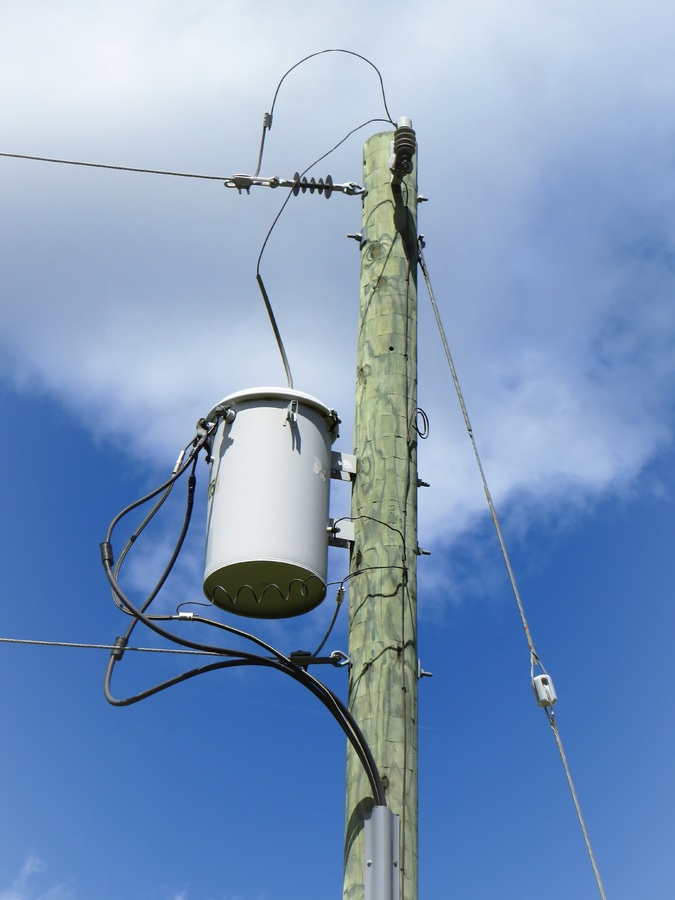
\includegraphics[width=0.75\textwidth]{fig/lec04/Transformer_rural_pole.jpg}
				\caption{Transformer integrated at a utility pole (source: \href{https://pxhere.com/en/photo/795672}{pxhere.com}, public domain)}
			\end{figure}
		\end{column}
		\end{columns}
\end{frame}

%%%%%%%%%%%%%%%%%%%%%%%%%%%%%%%%%%%%%%%%%%%%%%%%%%%%%%%%%%%%%
%% Examples of transformers %%
%%%%%%%%%%%%%%%%%%%%%%%%%%%%%%%%%%%%%%%%%%%%%%%%%%%%%%%%%%%%%
\begin{frame}
	\frametitle{Examples of transformers}
	\begin{figure}
		\centering
		\begin{subfigure}[b]{0.49\textwidth}
			\centering
			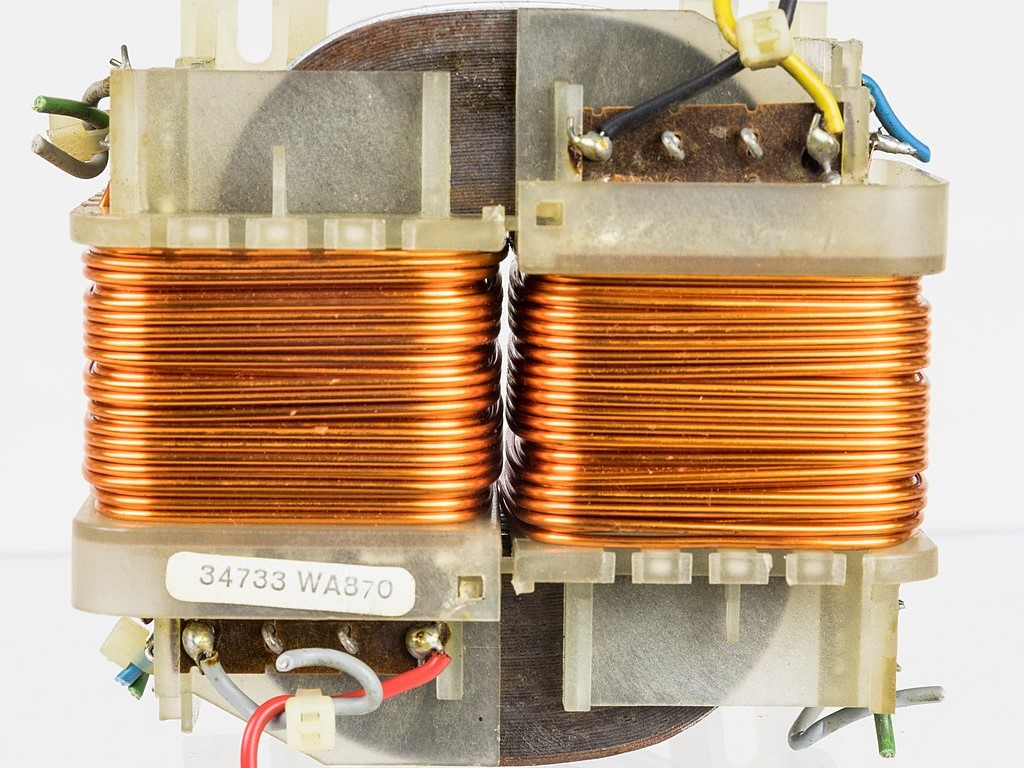
\includegraphics[width=0.45\textwidth]{fig/lec04/Power_supply_transformer.jpg}
			\caption{Power supply transformer (source: \href{https://commons.wikimedia.org/wiki/File:Philips_N4422_-_power_supply_transformer-2098.jpg}{Wikimedia Commons}, R.~Spekking, \href{https://creativecommons.org/licenses/by-sa/4.0/deed}{CC BY-SA 4.0})}
		\end{subfigure}
		\hfill
		\begin{subfigure}[b]{0.49\textwidth}
			\centering
			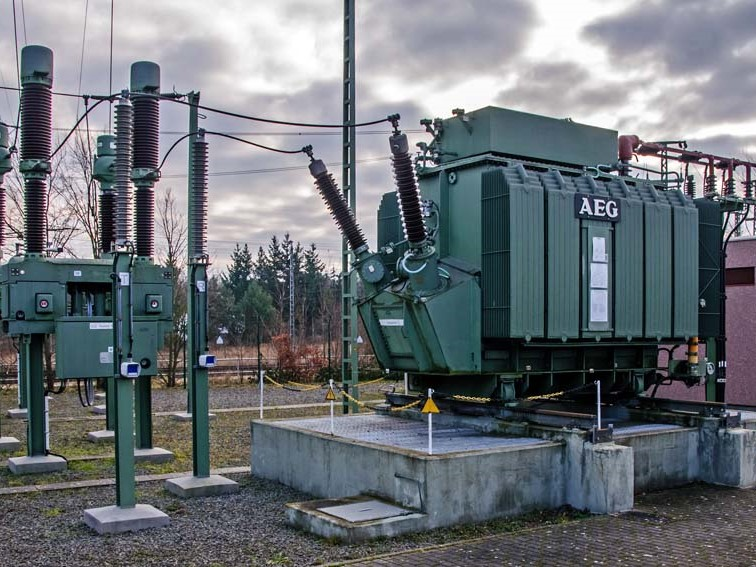
\includegraphics[width=0.45\textwidth]{fig/lec04/Single_phase_transformer.jpg}
			\caption{Single-phase transformer (source: \href{https://commons.wikimedia.org/wiki/File:DB_Unterwerk_Güsen,_Trafo_p.jpg}{Wikimedia Commons}, Georg, \href{https://creativecommons.org/licenses/by-sa/4.0/deed.en}{CC BY-SA 4.0})}
		\end{subfigure}
		\\
		\begin{subfigure}[b]{0.49\textwidth}
			\centering
			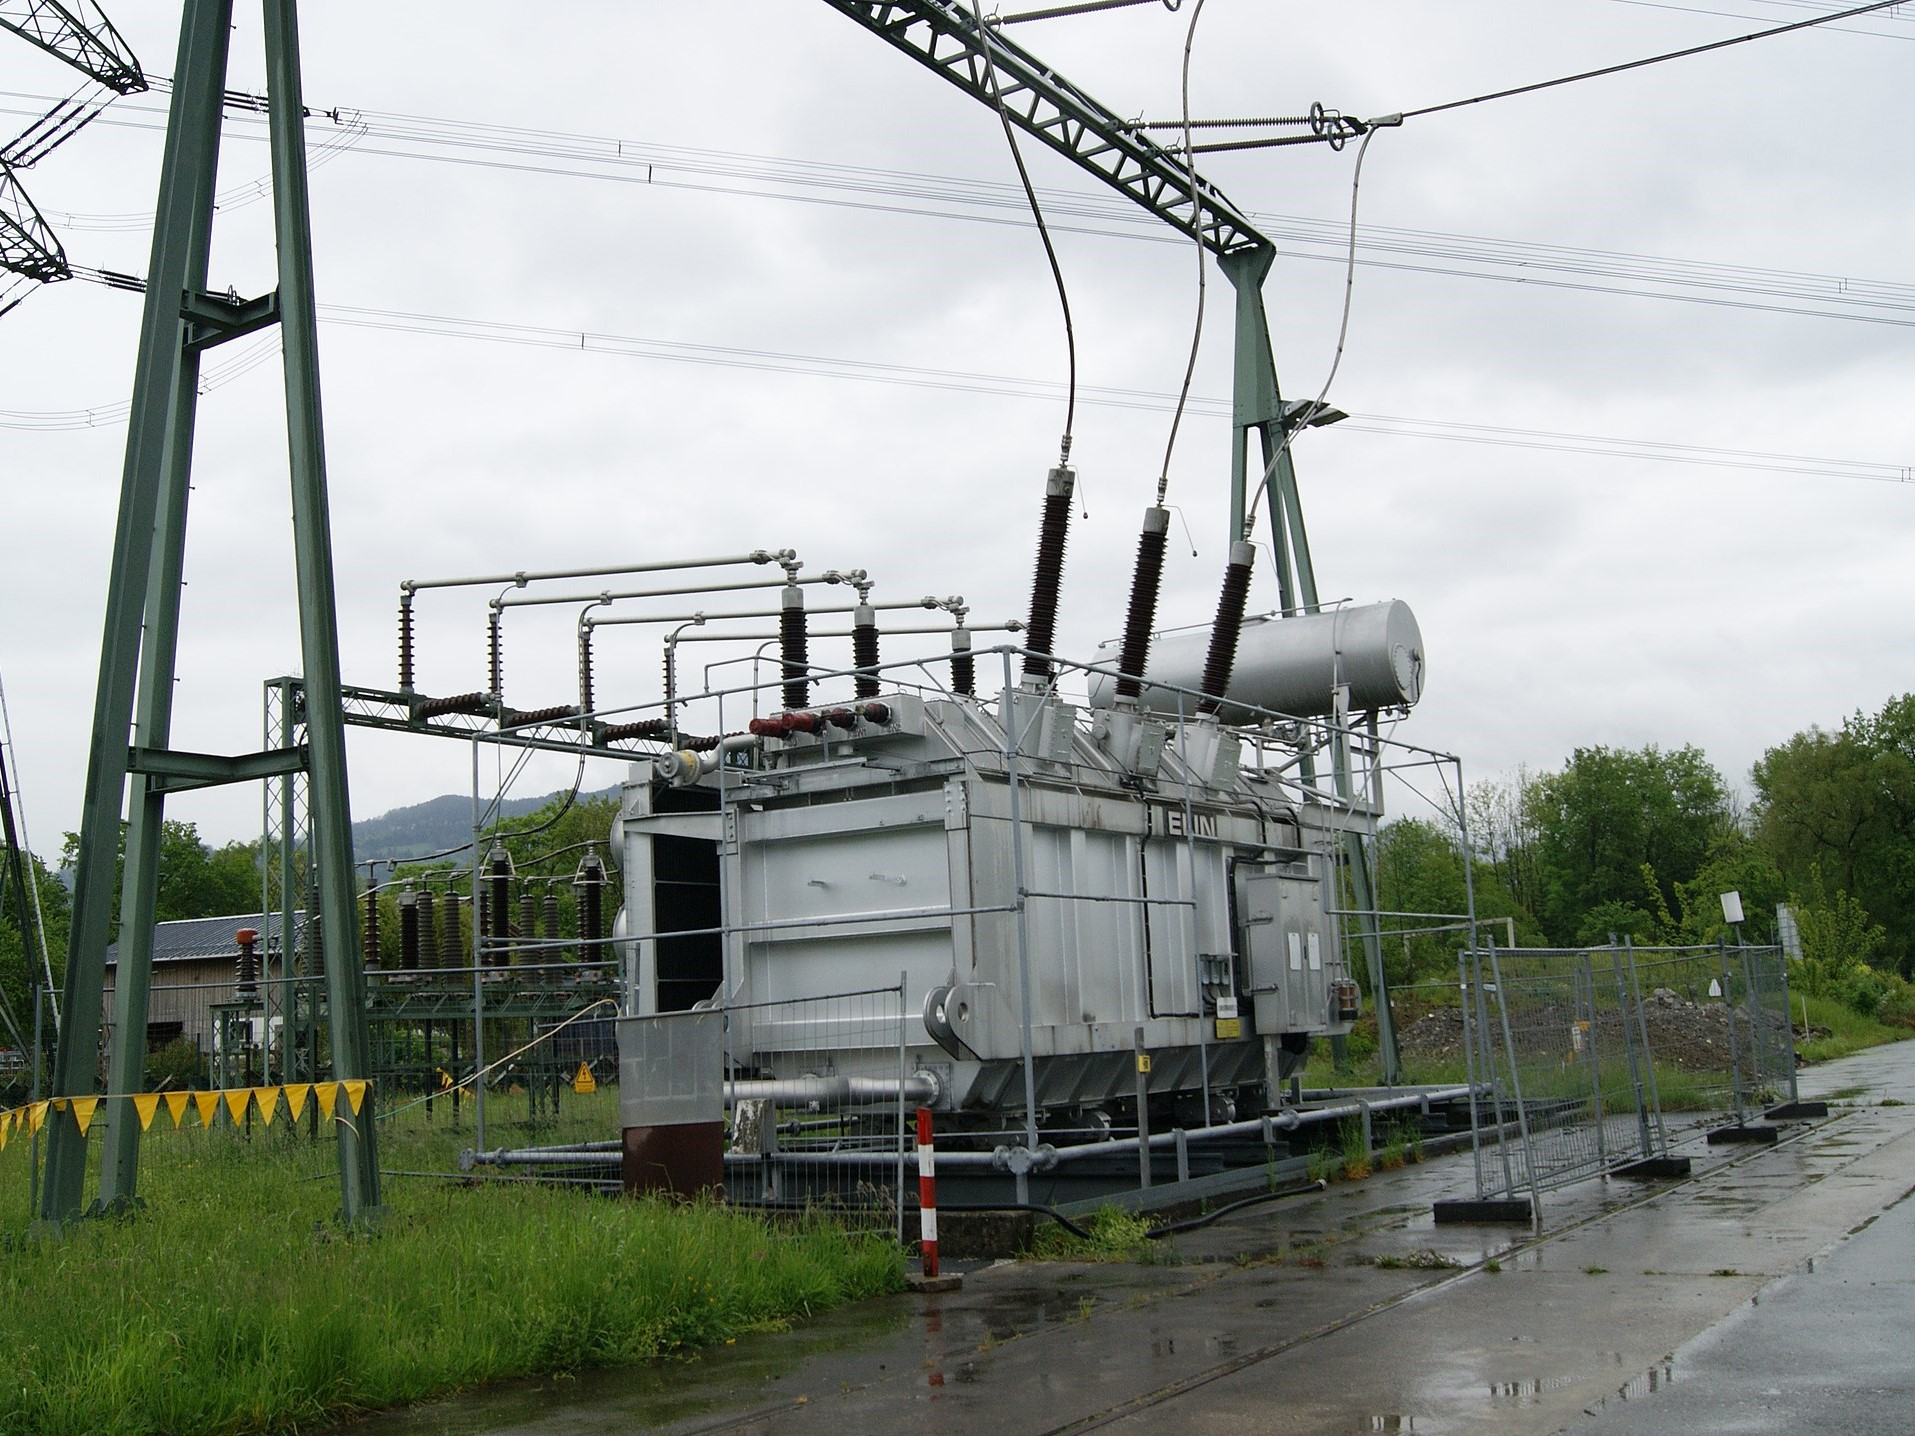
\includegraphics[width=0.45\textwidth]{fig/lec04/Three_phase_transformer.jpg}
			\caption{Three-phase transformer (source: \href{https://commons.wikimedia.org/wiki/File:Dornbirn-Umspannwerk_Werben-110kV_FS6-Anlage_Trafo_Elin_220-110kV-01ASD.jpg}{Wikimedia Commons}, Asurnipal, \href{https://creativecommons.org/licenses/by-sa/4.0/deed.en}{CC BY-SA 4.0})}
		\end{subfigure}
		\hfill
		\begin{subfigure}[b]{0.49\textwidth}
			\centering
			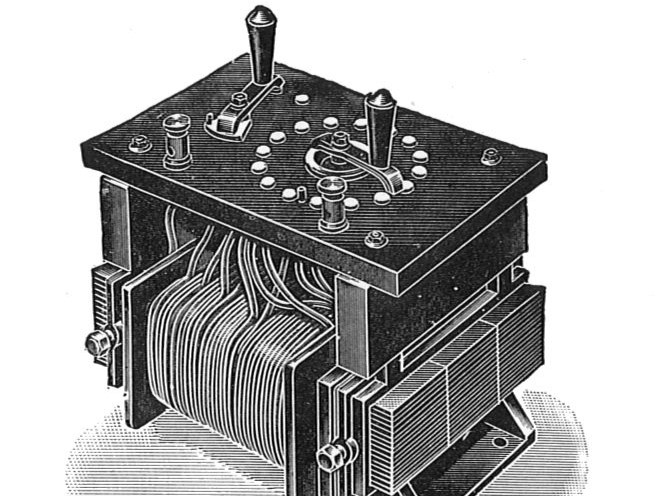
\includegraphics[width=0.45\textwidth]{fig/lec04/Tapped_transformer.jpg}
			\caption{Variable tapped transformer (source: \href{https://commons.wikimedia.org/wiki/File:Variable-tap_regulating_transformer_(Rankin_Kennedy,_Electrical_Installations,_Vol_II,_1909).jpg}{Wikimedia Commons}, public domain)}
		\end{subfigure}
		\caption*{Examples of transformers} 
        \label{fig:examples_transformers}
	\end{figure}
\end{frame}

%%%%%%%%%%%%%%%%%%%%%%%%%%%%%%%%%%%%%%%%%%%%%%%%%%%%%%%%%%%%%
%% Electromagnetic modeling of the single-phase transformer %%
%%%%%%%%%%%%%%%%%%%%%%%%%%%%%%%%%%%%%%%%%%%%%%%%%%%%%%%%%%%%%
\begin{frame}
	\frametitle{Electromagnetic modeling of the single-phase transformer}
    \begin{columns}
		\begin{column}{0.45\textwidth}
            Recap from \eqref{eq:flux_linkage_matrix_transformer}: for some given current $\bm{i}$, the flux linkages $\bm{\psi}$ in the transformer windings are
			\begin{equation*}
				\bm{\psi} = \begin{bmatrix} \psi_1 \\ \psi_2 \end{bmatrix} = \begin{bmatrix} L_1 & M \\ M & L_2 \end{bmatrix} \begin{bmatrix} i_1 \\ i_2 \end{bmatrix} = \bm{L}\bm{i}
			\end{equation*}
			where $L_1$ and $L_2$ are the self-inductances of the primary and secondary winding, respectively, and $M$ is the mutual inductance.
			\\[1em]
			Note: The above equation is an algebraic relation, that is, it is valid for any time instant $t$ and applies to both AC and DC excitation of the transformer. 
		\end{column}
        \hfill
		\begin{column}{0.525\textwidth}
			\begin{figure}
				\centering
				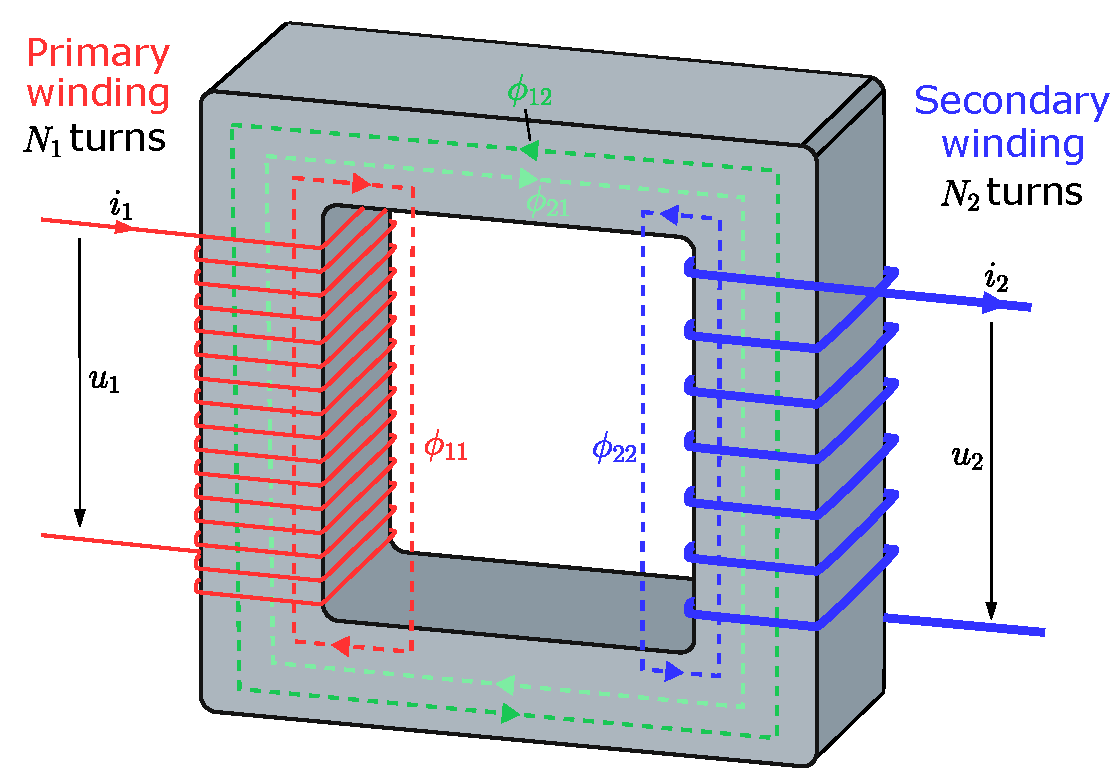
\includegraphics[height=0.575\textheight]{fig/lec02/Transformer3d_col3.pdf}
			\end{figure}
		\end{column}
		\end{columns}
\end{frame}

%%%%%%%%%%%%%%%%%%%%%%%%%%%%%%%%%%%%%%%%%%%%%%%%%%%%%%%%%%%%%
%% Dynamic modeling of the single-phase transformer %%
%%%%%%%%%%%%%%%%%%%%%%%%%%%%%%%%%%%%%%%%%%%%%%%%%%%%%%%%%%%%%
\begin{frame}
	\frametitle{Dynamic modeling of the single-phase transformer}
		The dynamic transformer behavior can be represented by the ECD in \figref{fig:General_transformer_ECD}, which also considers the internal resistances of the windings. Applying Faraday's law, the resulting differential equations are:
		\begin{align}
			u_1(t) = R_1 i_1(t) + \frac{\mathrm{d}\psi_1(t)}{\mathrm{d}t}, \qquad u_2(t) = R_2 i_2(t) + \frac{\mathrm{d}\psi_2(t)}{\mathrm{d}t}. \label{eq:transformer_differential_equations}
		\end{align}
		Inserting \eqref{eq:flux_linkage_matrix_transformer} delivers:
		\begin{align}
			u_1(t) = R_1 i_1(t) + L_1 \frac{\mathrm{d}i_1(t)}{\mathrm{d}t} + M \frac{\mathrm{d}i_2(t)}{\mathrm{d}t}, \qquad
			u_2(t) = R_2 i_2(t) + L_2 \frac{\mathrm{d}i_2(t)}{\mathrm{d}t} + M \frac{\mathrm{d}i_1(t)}{\mathrm{d}t}. \label{eq:transformer_differential_equations_2}
		\end{align}
		
\begin{figure}
\begin{columns}
	\begin{column}{0.55\textwidth}
            \centering
            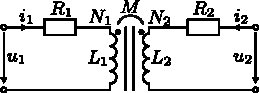
\includegraphics[width=0.8\textwidth]{fig/lec04/General_transformer_ECD.pdf}
    \end{column}
    \begin{column}{0.45\textwidth}
        \caption{\raggedright General equivalent circuit diagram (ECD) of a transformer (note: that both ports of the transformer are denoted in the load convention reference frame which is an arbitrary representation decision).}
		\label{fig:General_transformer_ECD}
    \end{column}
\end{columns}
\end{figure}
\end{frame}

%%%%%%%%%%%%%%%%%%%%%%%%%%%%%%%%%%%%%%%%%%%%%%%%%%%%%%%%%%%%%
%% Dynamic modeling of the single-phase transformer (cont.) %%
%%%%%%%%%%%%%%%%%%%%%%%%%%%%%%%%%%%%%%%%%%%%%%%%%%%%%%%%%%%%%
\begin{frame}
	\frametitle{Dynamic modeling of the single-phase transformer (cont.)}
		The model \eqref{eq:transformer_differential_equations_2} can be represented by the T-type ECD in \figref{fig:Transformer_T_ECD}. It may be noted that $L_1-M$ and $L_2-M$ can have negative values due to the model representation. 
		\\[1em]
		By rewritting \eqref{eq:transformer_differential_equations_2}, we can also write the dynamic transformer model in vector-matrix form:
		\begin{equation}
			\begin{bmatrix}	u_1(t)\\u_2(t) \end{bmatrix} = \bm{u}(t) = \begin{bmatrix} R_1 & 0 \\ 0 & R_2 \end{bmatrix} \begin{bmatrix} i_1(t)\\i_2(t) \end{bmatrix} + \begin{bmatrix} L_1 & M \\ M & L_2 \end{bmatrix} \frac{\mathrm{d}}{\mathrm{d}t} \begin{bmatrix} i_1(t)\\i_2(t) \end{bmatrix} = \bm{R}\bm{i}(t) + \bm{L}\frac{\mathrm{d}}{\mathrm{d}t}\bm{i}(t).  
			\label{eq:transformer_differential_equations_matrix_form}
		\end{equation}
\begin{figure}
\begin{columns}
	\begin{column}{0.55\textwidth}
            \centering
            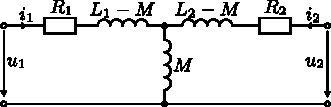
\includegraphics[width=0.9\textwidth]{fig/lec04/Transformer_T_ECD.pdf}
    \end{column}
    \begin{column}{0.45\textwidth}
        \caption{\raggedright T-type ECD of a transformer}
		\label{fig:Transformer_T_ECD}
    \end{column}
\end{columns}
\end{figure}
\end{frame}

%%%%%%%%%%%%%%%%%%%%%%%%%%%%%%%%%%%%%%%%%%%%%%%%%%%%%%%%%%%%%
%% Dynamic modeling of the single-phase transformer (cont.) %%
%%%%%%%%%%%%%%%%%%%%%%%%%%%%%%%%%%%%%%%%%%%%%%%%%%%%%%%%%%%%%
\begin{frame}
	\frametitle{Dynamic modeling of the single-phase transformer (cont.)}
		Rearranging \eqref{eq:transformer_differential_equations_matrix_form} gives the state-space representation of the transformer model
		\begin{equation}
			\frac{\mathrm{d}}{\mathrm{d}t}\bm{i}(t) = \bm{L}^{-1}\left(\bm{u}(t)-\bm{R}\bm{i}(t) \right)
			\label{eq:transformer_state_space_01}
		\end{equation}
		with
		$$ \renewcommand*{\arraystretch}{1.3} \bm{L}^{-1} = \frac{1}{L_1L_2 - M^2} \begin{bmatrix} L_2 & -M \\ -M & L_1 \end{bmatrix} = \frac{1}{\sigma} \begin{bmatrix} \frac{1}{L_1} &  \frac{-M}{L_1 L_2} \\ \frac{-M}{L_1 L_2} & \frac{1}{L_2} \end{bmatrix}.$$
		Above, $\sigma$ is the leakage coefficient defined as (compare also \eqref{eq:coupling_coefficient})
		\begin{equation}
			\sigma = \frac{L_1 L_2 -M^2}{L_1 L_2 } = 1 - \frac{M^2}{ L_1 L_2} = 1 - k^2 .
		\end{equation}
		Finally, the state-space representation of the transformer model is
		\begin{equation}
			\renewcommand*{\arraystretch}{1.3} 
			\frac{\mathrm{d}}{\mathrm{d}t}\bm{i}(t) = \begin{bmatrix} -\frac{R_1}{\sigma L_1} & \frac{R_2 M}{\sigma L_1 L_2} \\ \frac{R_1 M}{\sigma L_1 L_2} & -\frac{R_2}{\sigma L_1} \end{bmatrix} \bm{i}(t) + \begin{bmatrix} \frac{1}{\sigma L_1} & -\frac{M}{\sigma L_1 L_2} \\ -\frac{M}{\sigma L_1 L_2} & \frac{1}{\sigma L_2} \end{bmatrix} \bm{u}(t) = \bm{A} \bm{i}(t) + \bm{B} \bm{u}(t) .	 
			\label{eq:transformer_state_space_02}
		\end{equation}
\end{frame}

%%%%%%%%%%%%%%%%%%%%%%%%%%%%%%%%%%%%%%%%%%%%%%%%%%%%%%%%%%%%%
%% Steady-state of the single-phase transformer %%
%%%%%%%%%%%%%%%%%%%%%%%%%%%%%%%%%%%%%%%%%%%%%%%%%%%%%%%%%%%%%
\begin{frame}
	\frametitle{Steady-state modeling of the single-phase transformer}
		Assuming that the transformer operates in steady state and that all quantities are sinusoidal, the state-space model \eqref{eq:transformer_state_space_02} can be simplified and represented by complex phasors:
			$$x(t) = \hat{x} \cos(\omega_\mathrm{el} t+ \varphi_{\mathrm{x}}) = \mathrm{Re}\left\{\hat{x} e^{\iu (\omega_\mathrm{el} t + \varphi_{\mathrm{x}})}\right\}= \mathrm{Re}\left\{\underline{X} e^{\iu \omega_\mathrm{el} t}\right\}.$$
		From \eqref{eq:transformer_differential_equations_matrix_form} we recieve
		\begin{align}
			\bm{\underline{U}} = \begin{bmatrix} \underline{U}_1 \\ \underline{U}_2 \end{bmatrix} = \bm{R}\bm{\underline{I}} + \iu \omega_\mathrm{el} \bm{L}\bm{\underline{I}} = \bm{\underline{Z}}\, \bm{\underline{I} } = \begin{bmatrix} R_1 + \iu \omega_\mathrm{el} L_1 & \iu \omega_\mathrm{el} M \\ \iu \omega_\mathrm{el} M & R_2 + \iu \omega_\mathrm{el} L_2 \end{bmatrix} \begin{bmatrix} \underline{I}_1 \\ \underline{I}_2 \end{bmatrix}.
		\end{align}
		For some given $\bm{\underline{U}}$ we can calculate the current phasors $\bm{\underline{I}}$ (i.e., the steady-state current response) by solving:
		\begin{align}
			\renewcommand*{\arraystretch}{1.3} 
			\bm{\underline{I}} = \bm{\underline{Z}}^{-1} \bm{\underline{U}} .
			\label{eq:transformer_steady_state_current_response}
		\end{align}
\end{frame}

%%%%%%%%%%%%%%%%%%%%%%%%%%%%%%%%%%%%%%%%%%%%%%%%%%%%%%%%%%%%%
%% Transformation of the secondary side variables %%
%%%%%%%%%%%%%%%%%%%%%%%%%%%%%%%%%%%%%%%%%%%%%%%%%%%%%%%%%%%%%
\begin{frame}
	\frametitle{Transformation of the secondary side variables}
		Sometimes it can be helpful to (mathematically) transform the secondary side variables to ease the mathematical analysis. This can be done by introducing the transformation factor $\alpha$:
		\begin{equation}
			u_2' = \alpha u_2, \qquad i_2' = \frac{1}{\alpha} i_2.
		\end{equation}
		Here, $u_2'$ and $i_2'$ are the transformed secondary side voltage and current, respectively. The primary voltage equation reads
		\begin{equation}
			\begin{split}
			u_1(t) &= R_1 i_1(t) + L_1 \frac{\mathrm{d}i_1(t)}{\mathrm{d}t} + M \frac{\mathrm{d}i_2(t)}{\mathrm{d}t}  = R_1 i_1 (t)+ L_1 \frac{\mathrm{d}i_1(t)}{\mathrm{d}t}  + \alpha M \frac{\mathrm{d}i_2'(t)}{\mathrm{d}t}  \\&= R_1 i_1(t) + L_1 \frac{\mathrm{d}i_1(t)}{\mathrm{d}t} + M' \frac{\mathrm{d}i_2'(t)}{\mathrm{d}t}
		\end{split}
		\end{equation}
		with the transformed mutual inductance $M' = \alpha M$. 
\end{frame}

%%%%%%%%%%%%%%%%%%%%%%%%%%%%%%%%%%%%%%%%%%%%%%%%%%%%%%%%%%%%%
%% Transformation of the secondary side variables (cont.) %%
%%%%%%%%%%%%%%%%%%%%%%%%%%%%%%%%%%%%%%%%%%%%%%%%%%%%%%%%%%%%%
\begin{frame}
	\frametitle{Transformation of the secondary side variables (cont.)}
		Multiplying the secondary voltage equation with $\alpha$ gives 
		\begin{equation}
			\begin{split}
			\alpha  u_2(t)  &=  \alpha R_2 i_2(t) + \alpha L_2 \frac{\mathrm{d}i_2(t)}{\mathrm{d}t} + \alpha M \frac{\mathrm{d}i_1(t)}{\mathrm{d}t}\\
			\Leftrightarrow \quad u_2'(t) &= \alpha^2 R_2 i_2'(t) + \alpha^2 L_2 \frac{\mathrm{d}i_2'(t)}{\mathrm{d}t} + \alpha M \frac{\mathrm{d}i_1(t)}{\mathrm{d}t}\\
			\Leftrightarrow \quad u_2'(t) &=  R'_2 i_2'(t) + L'_2 \frac{\mathrm{d}i_2'(t)}{\mathrm{d}t} + M' \frac{\mathrm{d}i_1(t)}{\mathrm{d}t}
		\end{split}
		\end{equation}
		with the transformed resistance $R'_2 = \alpha^2 R_2$ and inductance $L'_2 = \alpha^2 L_2$.
		\begin{figure}
			\begin{columns}
				\begin{column}{0.55\textwidth}
						\centering
						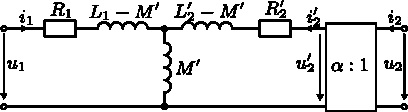
\includegraphics[width=0.99\textwidth]{fig/lec04/Transformer_T_ECD_gen_transf.pdf}
				\end{column}
				\begin{column}{0.45\textwidth}
					\caption{\raggedright T-type ECD of a transformer with transformed secondary side variables for some arbitrary transformation factor $\alpha$ (note that $k$ and $\sigma$ are transformation invariant, i.e., they also apply to the transformed model).}
					\label{fig:Transformer_T_ECD_gen_transf}
				\end{column}
			\end{columns}
		\end{figure}
\end{frame}

%%%%%%%%%%%%%%%%%%%%%%%%%%%%%%%%%%%%%%%%%%%%%%%%%%%%%%%%%%%%%
%% Transformation of the secondary side variables by the turn ratio %%
%%%%%%%%%%%%%%%%%%%%%%%%%%%%%%%%%%%%%%%%%%%%%%%%%%%%%%%%%%%%%
\begin{frame}
	\frametitle{Transformation of the secondary side variables by the turn ratio}
		
\end{frame}
